\chapter{The Restricted Full 3 Body Problem}
\label{RF3BP}
\graphicspath{{chapter-5/Images/}}

\section{Introduction}
In this chapter we will discuss the dynamics of the particle in motion around the binary asteroid system. We will consider that this particle in motion around the binary system is massless (basically its mass is negligibly small compared to the mass of either of the asteroids in the binary system) and so it will not affect the coupled dynamics of the binary asteroid system (see \Cref{F2BP}) itself. This particular problem in astrodynamics is referred to as the \textit{Restricted Full Three-Body Problem}. The \textit{Restricted} term refers to the fact that we have considered the third body, the orbiting particle in this case, to be massless. The \textit{Full} refers to the fact that the motion of the two primaries in the three-body problem, in this case the two primaries are the two asteroids, has not been simplified. We discussed the high-fidelity full two-body problem in \Cref{F2BP}. As always, our main focus would be on discussing the three body problem for the case where the asteroids are modeled as two polyhedrons, but a brief discussion on the three body problem for other binary asteroid models (as discussed previously in \Cref{F2BP}) will also be presented in this chapter.

\subsection{Circular Restricted Three-Body Problem}
\label{CRTBP}
The circular restricted three-body problem is a classic and fundamental astrodynamics problem. The acceleration of the third particle, in orbital motion around the two primaries (where the primaries, along with the third body, are all point masses), is derived from the gradient of the gravitational potential function \textit{U}. In the barycentric rotating frame, the equations of motion are expressed as follows \cite{chappaz}:
\begin{equation}
\label{crtbp_eom}
\ddot{\rho} + 2\omega \times \dot{\rho} + \omega \times (\omega \times \rho) + \dot{\omega} \times \rho = \frac{\partial U}{\partial \rho}
\end{equation}
%
In the above non-normalized equations of motion, the term \textit{U} combines the gravitational potential of both the primary and secondary body, $\rho$ specifies the position vector of the orbiting particle, defined in the barycentric rotating reference frame, $\omega$ is the angular velocity of the rotating two-body system, defined in the barycentric rotating reference frame.

\subsection{Sphere-Ellipsoid Restricted Three-Body Problem}
\label{SERTBP}
The orbital motion of the particle is modeled assuming that the primary and secondary are modeled as an ellipsoid and sphere respectively. The three-body geometry is depicted in \Cref{fig:sertbp} \cite{chappaz}:
\begin{figure}[h]
\centering
\captionsetup{justification=centering}
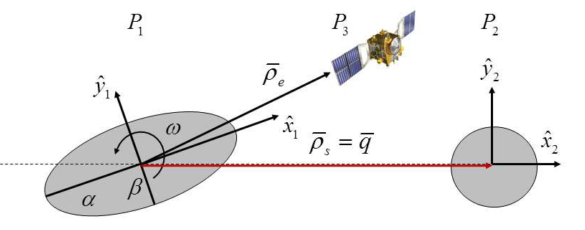
\includegraphics[scale=0.8]{sertbp.png}
\caption{Geometry of the Sphere-Ellipsoid restricted three-body problem \cite{chappaz}.}
\label{fig:sertbp}
\end{figure}
\FloatBarrier
%
Note that the position vector of the orbiting particle or spacecraft is defined in the body-fixed frame of the ellipsoid, denoted by the symbol $\rho_e$. The vector $\rho_s$ in \Cref{fig:sertbp} denotes the position of the centre of mass of the sphere with respect to the ellipsoid body-fixed frame. The equation of motion for the massless third particle is given as \cite{chappaz}:
\begin{equation}
\label{sertbp_eom}
\ddot{\rho_e} + 2\omega \times \dot{\rho_e} + \omega \times (\omega \times \rho_e) + \dot{\omega} \times \rho_e = \frac{\partial U_{SE}}{\partial \rho_e} + \frac{\partial U_{e1}}{\partial \rho_s}
\end{equation}
%
where $\omega$ is the angular rate of the ellipsoid. The term $U_{SE}$ is defined as $U_{SE} = \mu U_s + (1-\mu)U_{e1}$ where $U_s$ and $U_{e1}$ are the gravitational potential of the sphere and ellipsoid respectively. The term $\mu$ is the mass parameter of the system defined as $\mu = m_2/(m_1 + m_2)$ where $m_1$ and $m_2$ are the masses of the primary and secondary asteroid,  respectively, in the binary system \cite{chappaz}.

\subsection{Ellipsoid-Ellipsoid Restricted Three-Body Problem}
\label{EERTBP}
Here, the motion of the massless particle is computed assuming that the binary system is comprised of two ellipsoids. The geometry for this system is depicted in \Cref{fig:eertbp}:
\begin{figure}[h]
\centering
\captionsetup{justification=centering}
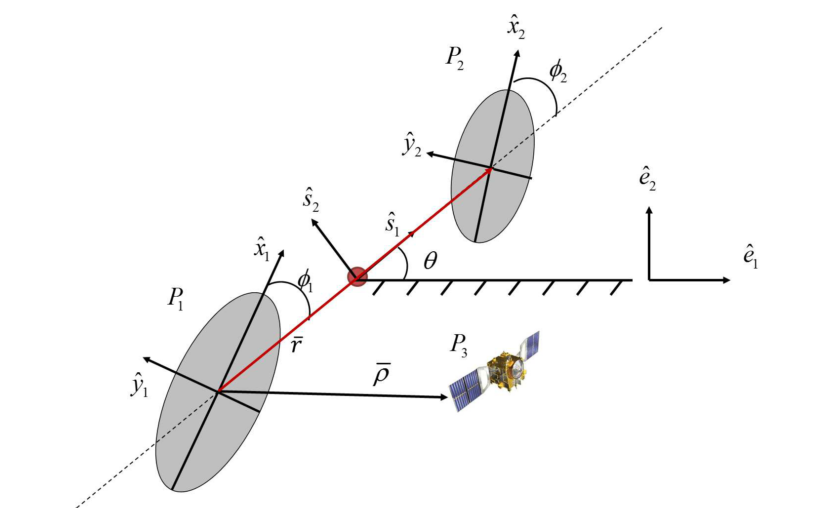
\includegraphics[scale=0.5]{eertbp.png}
\caption{Geometry of the Ellipsoid-Ellipsoid restricted three-body problem \cite{chappaz}.}
\label{fig:eertbp}
\end{figure}
\FloatBarrier
%
The position vector of the spacecraft is defined relative to the primary asteroid in the binary system and expressed in the inertial reference frame. The equation describing the motion of the third particle, in the inertial reference frame, is given as follows \cite{chappaz}:
\begin{equation}
\label{eertbp_eom}
\ddot{\rho} = \frac{\partial U_{EE}}{\partial \rho}
\end{equation}
%
The gravitational potential term $U_{EE}$ is computed as $U_{EE} = (1-\mu)U_{e1} + \mu U_{e2}$, where, $\mu$ is the mass parameter and is computed the same way as described in \Cref{SERTBP}. The terms $U_{e1}$ and $U_{e2}$ denote the potential of the primary and secondary ellipsoids in the binary system \cite{chappaz}.

\section{Polyhedron-Polyhedron Restricted Full Three-Body Problem}
\label{PPRFTBP}
Herein, we will focus more on the discussion of the equation of motion for the restricted full three-body problem assuming that the binary system is modeled as two polyhedrons. We begin by first defining the non-dimensional equation of motion. The reference frame under consideration is fixed to the rotating primary asteroid in the binary system (implying that the reference frame is rotating with the same angular velocity vector as the primary asteroid) but the frame's origin is fixed to the binary system's barycenter. For future reference, let's call this frame \textbf{RF1}. The equation of motion for a massless particle in \textbf{RF1} can be stated as follows \cite{dan_tbp}:
\begin{equation}
\label{eom1}
\ddot{\rho} + 2\Omega \times \dot{\rho} + \dot{\Omega} \times \rho + \Omega \times (\Omega \times \rho) = \frac{\partial U_{12}}{\partial \rho}
\end{equation}
%
where $\Omega$ is the angular rate of the primary asteroid defined in \textbf{RF1} or equivalently, in the primary asteroid's own frame. The term $\rho$ is the position vector of the particle, defined and originating from \textbf{RF1}. The potential term $U_{12}$ will be defined later. Now let's define a second reference frame which is fixed to the primary asteroid and also has its origin fixed to the centre of mass of the asteroid body. We will call this frame \textbf{RF2}. The equation of motion for a massless particle in this frame is defined as follows \cite{fahn_phd}:
\begin{equation}
\label{eom2}
\ddot{\rho} + 2\Omega \times \dot{\rho} + \dot{\Omega} \times \rho + \Omega \times (\Omega \times \rho) + \ddot{r}_1 = \frac{\partial U_{12}}{\partial \rho}
\end{equation}
%
where $\ddot{r}_1$ denotes the inertial acceleration of the centroid of the primary asteroid. The vector $\rho$ is still computed from the binary barycentre to the orbiting particle but expressed in \textbf{RF2}. We normalize the equation of motion for the third particle by considering a new unit for length, mass and time. For length \textit{L} we choose the largest dimension of the primary asteroid, for mass we can choose the total mass of the binary system i.e. $m_T = m_1 + m_2$, and for time we can choose the mean motion for the aforementioned new units of mass and length i.e. $n = \sqrt{G(m_1 + m_2)/L^3}$ \cite{fahn_phd}. Then the normalized position vector is given as $\varrho = \rho/L$ and the normalized angular velocity vector is given as $\omega = \Omega/n$ \cite{dan_tbp}. The normalized inertial position vector of the centroid of the primary asteroid will then be $R_1 = r_1/L$. The normalized equation of motion, as expressed in \textbf{RF2}, is stated as:
\begin{equation}
\label{eom3}
\ddot{\varrho} + 2\omega \times \dot{\varrho} + \dot{\omega} \times \varrho + \omega \times (\omega \times \varrho) + \ddot{R}_1 = \frac{\partial U_{12}}{\partial \varrho}
\end{equation}
%
The potential term $U_{12}$ is formulated with the same terminology and form as described for \Cref{polypot}. The expression is given as follows \cite{fahn_phd}:
\begin{equation}
\begin{aligned}
\label{U12}
U_{12} &= -G \sigma_1 \left[ -\frac{1}{2} \sum_{e\in edges_1} \overrightarrow{r}_{e1} \cdot E_{e1} \cdot \overrightarrow{r}_{e1} \cdot L_{e1} + \frac{1}{2} \sum_{f\in faces_1} \overrightarrow{r}_{f1} \cdot F_{f1} \cdot \overrightarrow{r}_{f1} \cdot w_{f1} \right] \\
 - & G \sigma_2 \left[ -\frac{1}{2} \sum_{e\in edges_2} \overrightarrow{r}_{e2} \cdot E_{e2} \cdot \overrightarrow{r}_{e2} \cdot L_{e2} + \frac{1}{2} \sum_{f\in faces_2} \overrightarrow{r}_{f2} \cdot F_{f2} \cdot \overrightarrow{r}_{f2} \cdot w_{f2} \right]
\end{aligned}
\end{equation}
%
where the subscripts 1 and 2 refer to the primary and secondary asteroid respectively; G is the normalized gravity constant and for the normalization terms currently being used, its value is unity; $\sigma_1$ and $\sigma_2$ are constant body densities for the two asteroids and they too are normalized \cite{fahn_phd}. The other terms in \Cref{U12} are defined properly in \Cref{polyhedron}. A very important thing to note here is that, no matter which reference frame is used to express the equation of motion for the third particle, its relative position vector, used in quantities $\overrightarrow{r}_e$, $\overrightarrow{r}_f$, $L_e$, and $w_f$, should be expressed in the body frame of the respective asteroid \cite{fahn_phd}. For this purpose we will define two attitude rotation matrices, one for each asteroid. $R_1$ will map from the body-fixed frame of the primary asteroid to the frame of the equation of motion (\textbf{RF1} or \textbf{RF2}) and similarly we define $R_2$ for the secondary asteroid. Of course, if the frame \textbf{RF2} is used to express the equation of motion then $R_1$ will be an identity matrix. The transpose of both $R_1$ and $R_2$ are used to express the relative position vector of the third particle in the respective body frames. These rotation matrices appear in the partial derivative of the potential term $U_{12}$ \cite{fahn_phd}.

The partial derivative of the potential $U_{12}$ is given as follows \cite{fahn_phd}:
\begin{equation}
\begin{aligned}
\label{U12_diff}
\frac{\partial U_{12}}{\partial \rho} &= -G \sigma_1 R_1 \left[ -\frac{1}{2} \sum_{e\in edges_1} E_{e1} \cdot \overrightarrow{r}_{e1} \cdot L_{e1} + \frac{1}{2} \sum_{f\in faces_1} F_{f1} \cdot \overrightarrow{r}_{f1} \cdot w_{f1} \right] \\
 - & G \sigma_2 R_2 \left[ -\frac{1}{2} \sum_{e\in edges_2} E_{e2} \cdot \overrightarrow{r}_{e2} \cdot L_{e2} + \frac{1}{2} \sum_{f\in faces_2} F_{f2} \cdot \overrightarrow{r}_{f2} \cdot w_{f2} \right]
\end{aligned}
\end{equation}
%
The second partial derivative of $U_{12}$ or the gravity gradient matrix is expressed as follows \cite{fahn_phd}:
\begin{equation}
\begin{aligned}
\label{U12_sec_diff}
\frac{\partial^2 U_{12}}{\partial \rho^2} &= -G \sigma_1 R_1 \left[ -\frac{1}{2} \sum_{e\in edges_1} E_{e1} \cdot L_{e1} + \frac{1}{2} \sum_{f\in faces_1} F_{f1} \cdot w_{f1} \right]R_1^T \\
 - & G \sigma_2 R_2 \left[ -\frac{1}{2} \sum_{e\in edges_2} E_{e2} \cdot L_{e2} + \frac{1}{2} \sum_{f\in faces_2} F_{f2} \cdot w_{f2} \right] R_2^T
\end{aligned}
\end{equation}
%
\subsection{Linearization}
\label{grav_lin}
The computation of gravitational attraction, as we can see from \Cref{U12_diff}, at a given field point in the vicinity of the binary asteroid system requires summation over all faces and edges of the two asteroids. A polyhedron, even at a small resolution, has hundreds of facets or faces and here we are dealing with two such polyhedrons which means that performing a summation over all the faces and edges will be computationally intensive. A linearization method, developed in \cite{stefaan_thesis}, helps in reducing the said computational load. For a given state, say $X_0$, we first compute the gravitational potential $U_{12}^{X0}$, the gravitational attraction $\partial U_{12}^{X0}/ \partial \rho$ and the gravity gradient matrix $\partial^2 U_{12}^{X0}/ \partial \rho^2$ using \Cref{U12}, \Cref{U12_diff} and \Cref{U12_sec_diff} respectively. Then, in the vicinity of this reference state $X_0$ we can compute the potential and its partial derivative for a state $X$ as follows \cite{stefaan_thesis}:
\begin{equation}
\label{u12_lin}
U_{12}^X = U_{12}^{X0} + (X - X_0) \frac{\partial U_{12}^{X0}}{\partial \rho} + (X - X_0)\frac{\partial^2 U_{12}^{X0}}{\partial \rho^2} (X - X_0)
\end{equation}
%
\begin{equation}
\label{u12_diff_lin}
\frac{\partial U_{12}^X}{\partial \rho} = \frac{\partial U_{12}^{X0}}{\partial \rho} + (X - X_0)\frac{\partial^2 U_{12}^{X0}}{\partial \rho^2}
\end{equation}
%
\Cref{u12_lin} and \Cref{u12_diff_lin} provide an approximation for the potential and its partial derivative only in the immediate neighborhood of the state $X_0$. For this reason, one should specify a certain limit $\Delta X_{max} = (X - X_0)_{max}$ wherein this approximation will be applied \cite{stefaan_thesis}. Following this method would definitely help in reducing the simulation time by a considerable amount.

\section{Conclusion}
In this chapter we began the discussion with models for the three-body problem. Except for the circular restricted three body problem, every other model presented in this chapter conforms to the restricted full 3-body problem formulation. The term \textit{Restricted} refers to the fact that the third body is modeled as a massless particle and the term \textit{Full} refers to the fact that the remaining two bodies in the problem have not been considered as point mass objects but rather the dynamics, both rotational and translational, of the bodies have been modeled considering their specific geometric shapes. The polyhedron-polyhedron restricted full three body problem has been discussed in more detail than the other models since it is the approach which has been chosen to study the long term orbital motion of a third particle due to the higher level of accuracy offered by it. This model is used not only to study the motion of a third particle around it but also to simulate the motion of the binary asteroids around each other. Expressions for the potential, gravitational attraction and the gravity gradient matrix were presented. A linearization approach to reduce the computational loads in calculating the potential and its derivatives was also presented in this chapter.
